% Options for packages loaded elsewhere
\PassOptionsToPackage{unicode}{hyperref}
\PassOptionsToPackage{hyphens}{url}
%
\documentclass[
]{book}
\usepackage{amsmath,amssymb}
\usepackage{lmodern}
\usepackage{iftex}
\ifPDFTeX
  \usepackage[T1]{fontenc}
  \usepackage[utf8]{inputenc}
  \usepackage{textcomp} % provide euro and other symbols
\else % if luatex or xetex
  \usepackage{unicode-math}
  \defaultfontfeatures{Scale=MatchLowercase}
  \defaultfontfeatures[\rmfamily]{Ligatures=TeX,Scale=1}
\fi
% Use upquote if available, for straight quotes in verbatim environments
\IfFileExists{upquote.sty}{\usepackage{upquote}}{}
\IfFileExists{microtype.sty}{% use microtype if available
  \usepackage[]{microtype}
  \UseMicrotypeSet[protrusion]{basicmath} % disable protrusion for tt fonts
}{}
\makeatletter
\@ifundefined{KOMAClassName}{% if non-KOMA class
  \IfFileExists{parskip.sty}{%
    \usepackage{parskip}
  }{% else
    \setlength{\parindent}{0pt}
    \setlength{\parskip}{6pt plus 2pt minus 1pt}}
}{% if KOMA class
  \KOMAoptions{parskip=half}}
\makeatother
\usepackage{xcolor}
\usepackage{color}
\usepackage{fancyvrb}
\newcommand{\VerbBar}{|}
\newcommand{\VERB}{\Verb[commandchars=\\\{\}]}
\DefineVerbatimEnvironment{Highlighting}{Verbatim}{commandchars=\\\{\}}
% Add ',fontsize=\small' for more characters per line
\usepackage{framed}
\definecolor{shadecolor}{RGB}{248,248,248}
\newenvironment{Shaded}{\begin{snugshade}}{\end{snugshade}}
\newcommand{\AlertTok}[1]{\textcolor[rgb]{0.94,0.16,0.16}{#1}}
\newcommand{\AnnotationTok}[1]{\textcolor[rgb]{0.56,0.35,0.01}{\textbf{\textit{#1}}}}
\newcommand{\AttributeTok}[1]{\textcolor[rgb]{0.77,0.63,0.00}{#1}}
\newcommand{\BaseNTok}[1]{\textcolor[rgb]{0.00,0.00,0.81}{#1}}
\newcommand{\BuiltInTok}[1]{#1}
\newcommand{\CharTok}[1]{\textcolor[rgb]{0.31,0.60,0.02}{#1}}
\newcommand{\CommentTok}[1]{\textcolor[rgb]{0.56,0.35,0.01}{\textit{#1}}}
\newcommand{\CommentVarTok}[1]{\textcolor[rgb]{0.56,0.35,0.01}{\textbf{\textit{#1}}}}
\newcommand{\ConstantTok}[1]{\textcolor[rgb]{0.00,0.00,0.00}{#1}}
\newcommand{\ControlFlowTok}[1]{\textcolor[rgb]{0.13,0.29,0.53}{\textbf{#1}}}
\newcommand{\DataTypeTok}[1]{\textcolor[rgb]{0.13,0.29,0.53}{#1}}
\newcommand{\DecValTok}[1]{\textcolor[rgb]{0.00,0.00,0.81}{#1}}
\newcommand{\DocumentationTok}[1]{\textcolor[rgb]{0.56,0.35,0.01}{\textbf{\textit{#1}}}}
\newcommand{\ErrorTok}[1]{\textcolor[rgb]{0.64,0.00,0.00}{\textbf{#1}}}
\newcommand{\ExtensionTok}[1]{#1}
\newcommand{\FloatTok}[1]{\textcolor[rgb]{0.00,0.00,0.81}{#1}}
\newcommand{\FunctionTok}[1]{\textcolor[rgb]{0.00,0.00,0.00}{#1}}
\newcommand{\ImportTok}[1]{#1}
\newcommand{\InformationTok}[1]{\textcolor[rgb]{0.56,0.35,0.01}{\textbf{\textit{#1}}}}
\newcommand{\KeywordTok}[1]{\textcolor[rgb]{0.13,0.29,0.53}{\textbf{#1}}}
\newcommand{\NormalTok}[1]{#1}
\newcommand{\OperatorTok}[1]{\textcolor[rgb]{0.81,0.36,0.00}{\textbf{#1}}}
\newcommand{\OtherTok}[1]{\textcolor[rgb]{0.56,0.35,0.01}{#1}}
\newcommand{\PreprocessorTok}[1]{\textcolor[rgb]{0.56,0.35,0.01}{\textit{#1}}}
\newcommand{\RegionMarkerTok}[1]{#1}
\newcommand{\SpecialCharTok}[1]{\textcolor[rgb]{0.00,0.00,0.00}{#1}}
\newcommand{\SpecialStringTok}[1]{\textcolor[rgb]{0.31,0.60,0.02}{#1}}
\newcommand{\StringTok}[1]{\textcolor[rgb]{0.31,0.60,0.02}{#1}}
\newcommand{\VariableTok}[1]{\textcolor[rgb]{0.00,0.00,0.00}{#1}}
\newcommand{\VerbatimStringTok}[1]{\textcolor[rgb]{0.31,0.60,0.02}{#1}}
\newcommand{\WarningTok}[1]{\textcolor[rgb]{0.56,0.35,0.01}{\textbf{\textit{#1}}}}
\usepackage{longtable,booktabs,array}
\usepackage{calc} % for calculating minipage widths
% Correct order of tables after \paragraph or \subparagraph
\usepackage{etoolbox}
\makeatletter
\patchcmd\longtable{\par}{\if@noskipsec\mbox{}\fi\par}{}{}
\makeatother
% Allow footnotes in longtable head/foot
\IfFileExists{footnotehyper.sty}{\usepackage{footnotehyper}}{\usepackage{footnote}}
\makesavenoteenv{longtable}
\usepackage{graphicx}
\makeatletter
\def\maxwidth{\ifdim\Gin@nat@width>\linewidth\linewidth\else\Gin@nat@width\fi}
\def\maxheight{\ifdim\Gin@nat@height>\textheight\textheight\else\Gin@nat@height\fi}
\makeatother
% Scale images if necessary, so that they will not overflow the page
% margins by default, and it is still possible to overwrite the defaults
% using explicit options in \includegraphics[width, height, ...]{}
\setkeys{Gin}{width=\maxwidth,height=\maxheight,keepaspectratio}
% Set default figure placement to htbp
\makeatletter
\def\fps@figure{htbp}
\makeatother
\setlength{\emergencystretch}{3em} % prevent overfull lines
\providecommand{\tightlist}{%
  \setlength{\itemsep}{0pt}\setlength{\parskip}{0pt}}
\setcounter{secnumdepth}{5}
\usepackage{booktabs}
\ifLuaTeX
  \usepackage{selnolig}  % disable illegal ligatures
\fi
\usepackage[]{natbib}
\bibliographystyle{plainnat}
\IfFileExists{bookmark.sty}{\usepackage{bookmark}}{\usepackage{hyperref}}
\IfFileExists{xurl.sty}{\usepackage{xurl}}{} % add URL line breaks if available
\urlstyle{same} % disable monospaced font for URLs
\hypersetup{
  pdftitle={MetaNet Tutorial},
  pdfauthor={Peng Chen},
  hidelinks,
  pdfcreator={LaTeX via pandoc}}

\title{MetaNet Tutorial}
\author{Peng Chen}
\date{2023-02-26}

\begin{document}
\maketitle

{
\setcounter{tocdepth}{1}
\tableofcontents
}
\hypertarget{about}{%
\chapter{About}\label{about}}

\hypertarget{install}{%
\section{Install}\label{install}}

MetaNet is a comprehensive network analysis package, especially in various omics.

the latest version can be found in \url{https://github.com/Asa12138/MetaNet}.

for some data manipulation, we recommend to use \texttt{dplyr}

\begin{Shaded}
\begin{Highlighting}[]
\NormalTok{remotes}\SpecialCharTok{::}\FunctionTok{install\_github}\NormalTok{(}\StringTok{\textquotesingle{}Asa12138/pcutils\textquotesingle{}}\NormalTok{)}
\NormalTok{remotes}\SpecialCharTok{::}\FunctionTok{install\_github}\NormalTok{(}\StringTok{\textquotesingle{}Asa12138/MetaNet\textquotesingle{}}\NormalTok{,}\AttributeTok{dependencies=}\NormalTok{T)}
\FunctionTok{library}\NormalTok{(MetaNet)}
\FunctionTok{library}\NormalTok{(igraph)}
\CommentTok{\#data manipulation}
\FunctionTok{library}\NormalTok{(dplyr)}
\end{Highlighting}
\end{Shaded}

\begin{Shaded}
\begin{Highlighting}[]
\FunctionTok{sessionInfo}\NormalTok{()}
\end{Highlighting}
\end{Shaded}

\begin{verbatim}
## R version 4.2.2 (2022-10-31)
## Platform: aarch64-apple-darwin20 (64-bit)
## Running under: macOS Ventura 13.0.1
## 
## Matrix products: default
## BLAS:   /Library/Frameworks/R.framework/Versions/4.2-arm64/Resources/lib/libRblas.0.dylib
## LAPACK: /Library/Frameworks/R.framework/Versions/4.2-arm64/Resources/lib/libRlapack.dylib
## 
## locale:
## [1] en_US.UTF-8/en_US.UTF-8/en_US.UTF-8/C/en_US.UTF-8/en_US.UTF-8
## 
## attached base packages:
## [1] stats     graphics  grDevices utils     datasets  methods   base     
## 
## loaded via a namespace (and not attached):
##  [1] bookdown_0.32   digest_0.6.31   lifecycle_1.0.3 magrittr_2.0.3 
##  [5] evaluate_0.19   rlang_1.0.6     stringi_1.7.8   cli_3.6.0      
##  [9] rstudioapi_0.14 vctrs_0.5.1     rmarkdown_2.19  tools_4.2.2    
## [13] stringr_1.5.0   glue_1.6.2      xfun_0.36       yaml_2.3.6     
## [17] fastmap_1.1.0   compiler_4.2.2  htmltools_0.5.4 knitr_1.41
\end{verbatim}

\hypertarget{introduction}{%
\chapter{Introduction}\label{introduction}}

\hypertarget{network}{%
\section{Network}\label{network}}

In mathematics,``networks'' are often referred to as ``graphs'',and the
mathematical field of graph research is called ``graph theory''.

The basic elements in a network graph are nodes and edges. When
constructing a network graph,the objects are called ``nodes'' (vertices or
nodes),and they are usually drawn as points; the connections between
nodes are called ``edges'' (edges). or links),and they are usually drawn
as lines between points.

We Can be divide into directed and undirected networks,weighted and
unweighted networks according to the edges.

\hypertarget{network-in-omics}{%
\section{Network in omics}\label{network-in-omics}}

Networks can represent various systems in the real world,and have many
applications in biological research,especially in systems biology: gene
expression regulatory networks,metabolic networks,ecosystem space
networks,microbial co-occurrence networks,protein interaction
networks,etc.

\begin{figure}
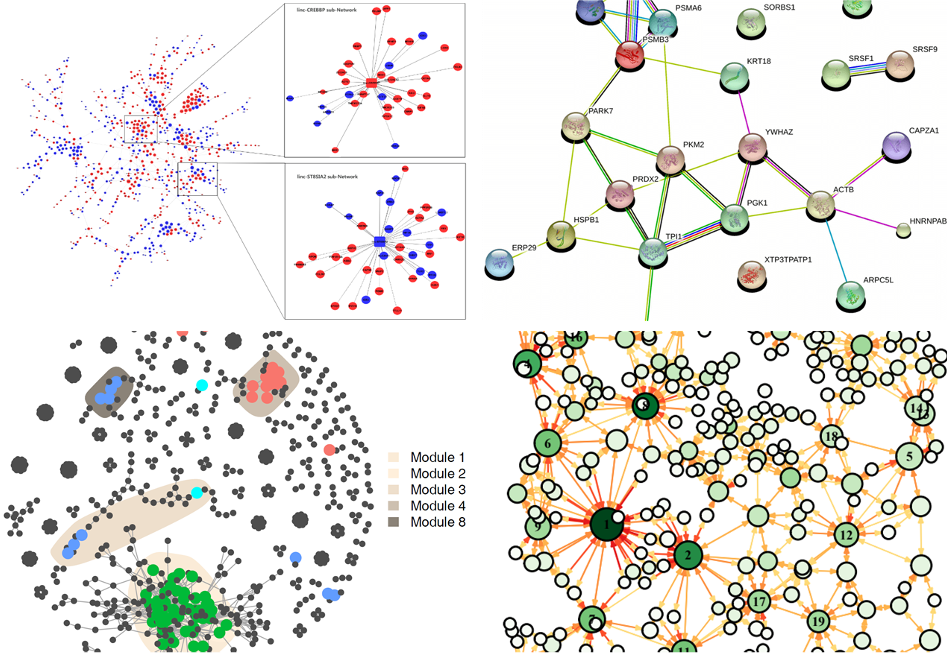
\includegraphics[width=13.15in]{images/1-1.net_application} \caption{Applications of network in biology}\label{fig:unnamed-chunk-4}
\end{figure}

WGCNA

Co-occurrence networks

PPI

\hypertarget{software}{%
\section{Software}\label{software}}

\begin{itemize}
\item
  R: igraph (\url{https://igraph.org/}), network
\item
  Python: networkx (\url{https://pypi.org/project/networkx/} )
\item
  Pajek (\url{http://vlado.fmf.uni-lj.si/pub/networks/pajek/} )
\item
  Cytoscape (\url{https://cytoscape.org/} )
\item
  Gephi (\url{https://gephi.org/} )
\end{itemize}

\hypertarget{metanet}{%
\section{MetaNet}\label{metanet}}

\textbf{MetaNet} is a comprehensive network analysis package.

\begin{itemize}
\item
  Calculate correlation network quickly, accelerate lots of analysis
  by parallel computing.
\item
  Support for multi-omics data, search sub-nets fluently.
\item
  Handle bigger data, more than 10,000 nodes in each omics.
\item
  Offer various layout method for multi-omics network and some
  interfaces to other software (Gephi, Cytoscape, ggplot), easy to
  visualize.
\item
  Provide comprehensive topology indexes calculation,including
  ecological network stability.
\end{itemize}

\hypertarget{construction}{%
\chapter{Construction}\label{construction}}

\hypertarget{normalization}{%
\section{Pre-processing}\label{normalization}}

The \texttt{trans()} function contains many normalization methods, suitable for pre-processing of different omics, some refer to \texttt{vegan::decostand()} (\citet{R-vegan}).

\begin{longtable}[]{@{}
  >{\raggedright\arraybackslash}p{(\columnwidth - 2\tabcolsep) * \real{0.0838}}
  >{\raggedright\arraybackslash}p{(\columnwidth - 2\tabcolsep) * \real{0.9162}}@{}}
\caption{Table 3.1: Normalization methods used in omics.}\tabularnewline
\toprule()
\endhead
\textbf{Method} & \textbf{Description} \\
cpm & Counts per million \\
minmax & linear transfer to (min, max) \\
acpm & Counts per million, then asinh transfer \\
log1 & log(n+1) transformat \\
total & divide by total \\
max & divide by maximum \\
frequency & divide by total and multiply by the number of non-zero items, so that the average of non-zero entries is one \\
normalize & make margin sum of squares equal to one \\
range & standardize values into range 0 ... 1 (same to \texttt{minmax(0,1)}). If all values are constant, they will be transformed to 0. \\
rank & rank replaces abundance values by their increasing ranks leaving zeros unchanged \\
rank, rrank & rank replaces abundance values by their increasing ranks leaving zeros unchanged, and rrank is similar but uses relative ranks with maximum 1 \\
pa & scale x to presence/absence scale (0/1). \\
standardize & scale x to zero mean and unit variance \\
hellinger & square root of method = ``total'' \\
log & logarithmic transformation as suggested by Anderson et al.~(2006): logb(x)+1 for x\textgreater0, where bb is the base of the logarithm; zeros are left as zeros. \\
alr & Additive log ratio (``alr'') transformation (Aitchison 1986) reduces data skewness and compositionality bias.

\(alr=[log\frac{x_1}{x_D},…,log\frac{x_{D-1}}{x_D}]\) \\
clr & centered log ratio (``clr'') transformation proposed by Aitchison (1986) reduces data skewness and compositionality bias.

\(clr=log\frac{x_r}{g(x_r)}\) \\
rclr & robust clr (``rclr'') is similar to regular clr (see above) but allows data that contains zeroes.

\(rclr=log\frac{x_r}{g(x_r>0)}\) \\
\bottomrule()
\end{longtable}

\begin{Shaded}
\begin{Highlighting}[]
\FunctionTok{library}\NormalTok{(MetaNet)}
\FunctionTok{data}\NormalTok{(otutab)}
\CommentTok{\#trans(otutab,method="cpm")\%\textgreater{}\%head()}
\FunctionTok{trans}\NormalTok{(otutab,}\AttributeTok{method=}\StringTok{"log1"}\NormalTok{)}\SpecialCharTok{\%\textgreater{}\%}\FunctionTok{head}\NormalTok{(}\DecValTok{4}\NormalTok{)}
\end{Highlighting}
\end{Shaded}

\begin{verbatim}
##                                   NS1      NS2      NS3      NS4      NS5
## s__un_f__Thermomonosporaceae 6.996681 7.560601 6.698268 7.211557 6.970730
## s__Pelomonas_puraquae        7.582229 7.118826 7.767687 7.712891 7.973844
## s__Rhizobacter_bergeniae     6.378426 6.129050 6.791221 6.804615 7.112327
## s__Flavobacterium_terrae     5.501258 5.459586 7.501634 6.513230 7.276556
##                                   NS6      WS1      WS2      WS3      WS4
## s__un_f__Thermomonosporaceae 6.976348 7.133296 7.376508 7.193686 6.848005
## s__Pelomonas_puraquae        7.512071 6.469250 6.206576 7.115582 7.158514
## s__Rhizobacter_bergeniae     6.749931 6.405228 6.154858 6.976348 6.936343
## s__Flavobacterium_terrae     6.198479 5.765191 7.563720 7.309212 6.903747
##                                   WS5      WS6      CS1      CS2      CS3
## s__un_f__Thermomonosporaceae 7.118016 6.919684 7.746733 7.831617 7.444249
## s__Pelomonas_puraquae        6.860664 6.455199 7.174724 7.324490 6.739337
## s__Rhizobacter_bergeniae     6.741701 6.508769 6.937314 7.497207 6.910751
## s__Flavobacterium_terrae     6.359574 5.886104 6.985642 7.105786 6.626718
##                                   CS4      CS5      CS6
## s__un_f__Thermomonosporaceae 7.588830 7.266827 7.331715
## s__Pelomonas_puraquae        7.029088 7.302496 7.069023
## s__Rhizobacter_bergeniae     7.090910 7.085901 6.637258
## s__Flavobacterium_terrae     6.049733 6.940222 7.253470
\end{verbatim}

\texttt{guolv()} and \texttt{hebing()} functions provide can help filter or aggregate the omics data.

\hypertarget{pairwise-relationship}{%
\section{Pairwise relationship}\label{pairwise-relationship}}

How to determine the pairwise relationship, because the experimental data is generally relatively rare, we mainly relying on statistical inference.

At present, there are mainly two ways, the first one is based on similarity or correlation \citet{faustMicrobialInteractionsNetworks2012}. for example: Spearman, Pearson, Bray-Curtis\ldots{} based on abundance or incidence data, the similarity matrix between paired species can be calculated, and the randomized data can be used to repeatedly calculate the significance.Finally, meaningful similarities are retained in network.

The second way for networks is based on regression. Divide species into source and target, and use multiple regression to calculate the relationship between species.

Some tools use special methods to optimize the network construction, such as \textbf{SparCC}, etc.

\hypertarget{correlation}{%
\subsection{Correlation}\label{correlation}}

\textbf{Correlation} is a statistical term describing the degree to which two variables move in coordination with one-another.

Correlation calculation is the first step in all omics network analysis software, there are many method to get \(\rho\) and \(p\)-value. However, as the data size of omics grow larger and larger, many methods will become very time and computational resource consuming.

Here, we provide the \texttt{c\_net\_cal()} function for one single table or two tables to calculate correlation \textbf{fastly} (Figure \ref{fig:packages-comparison}), which will return a three elements list include \(\rho\), \(p\)-value and \(p\)-adjust.

\begin{Shaded}
\begin{Highlighting}[]
\CommentTok{\#single table}
\FunctionTok{t}\NormalTok{(otutab) }\OtherTok{{-}\textgreater{}}\NormalTok{ totu}
\FunctionTok{c\_net\_cal}\NormalTok{(totu,}\AttributeTok{method =} \StringTok{"spearman"}\NormalTok{, }\AttributeTok{filename =}\NormalTok{F,}\AttributeTok{p.adjust.method =} \ConstantTok{NULL}\NormalTok{) }\OtherTok{{-}\textgreater{}}\NormalTok{ corr}
\FunctionTok{str}\NormalTok{(corr)}
\end{Highlighting}
\end{Shaded}

\begin{verbatim}
## List of 3
##  $ r       : num [1:464, 1:464] 0 -0.2508 0.1847 0.0114 0.2095 ...
##   ..- attr(*, "dimnames")=List of 2
##   .. ..$ : chr [1:464] "s__un_f__Thermomonosporaceae" "s__Pelomonas_puraquae" "s__Rhizobacter_bergeniae" "s__Flavobacterium_terrae" ...
##   .. ..$ : chr [1:464] "s__un_f__Thermomonosporaceae" "s__Pelomonas_puraquae" "s__Rhizobacter_bergeniae" "s__Flavobacterium_terrae" ...
##  $ p.value : num [1:464, 1:464] 0 0.316 0.463 0.964 0.404 ...
##   ..- attr(*, "dimnames")=List of 2
##   .. ..$ : chr [1:464] "s__un_f__Thermomonosporaceae" "s__Pelomonas_puraquae" "s__Rhizobacter_bergeniae" "s__Flavobacterium_terrae" ...
##   .. ..$ : chr [1:464] "s__un_f__Thermomonosporaceae" "s__Pelomonas_puraquae" "s__Rhizobacter_bergeniae" "s__Flavobacterium_terrae" ...
##  $ p.adjust: num [1:464, 1:464] 0 0.316 0.463 0.964 0.404 ...
##   ..- attr(*, "dimnames")=List of 2
##   .. ..$ : chr [1:464] "s__un_f__Thermomonosporaceae" "s__Pelomonas_puraquae" "s__Rhizobacter_bergeniae" "s__Flavobacterium_terrae" ...
##   .. ..$ : chr [1:464] "s__un_f__Thermomonosporaceae" "s__Pelomonas_puraquae" "s__Rhizobacter_bergeniae" "s__Flavobacterium_terrae" ...
\end{verbatim}

\begin{Shaded}
\begin{Highlighting}[]
\CommentTok{\#two tables}
\NormalTok{metadata[,}\DecValTok{3}\SpecialCharTok{:}\DecValTok{10}\NormalTok{] }\OtherTok{{-}\textgreater{}}\NormalTok{ env}
\FunctionTok{c\_net\_cal}\NormalTok{(totu,env,}\AttributeTok{method =} \StringTok{"spearman"}\NormalTok{, }\AttributeTok{filename =}\NormalTok{F,}\AttributeTok{p.adjust.method =} \ConstantTok{NULL}\NormalTok{) }\OtherTok{{-}\textgreater{}}\NormalTok{ corr2}
\FunctionTok{str}\NormalTok{(corr2)}
\end{Highlighting}
\end{Shaded}

\begin{verbatim}
## List of 3
##  $ r       : num [1:464, 1:8] 0.356 -0.5253 0.0918 -0.0114 -0.0196 ...
##   ..- attr(*, "dimnames")=List of 2
##   .. ..$ : chr [1:464] "s__un_f__Thermomonosporaceae" "s__Pelomonas_puraquae" "s__Rhizobacter_bergeniae" "s__Flavobacterium_terrae" ...
##   .. ..$ : chr [1:8] "env1" "env2" "env3" "env4" ...
##  $ p.value : num [1:464, 1:8] 0.147 0.0252 0.717 0.9643 0.9384 ...
##   ..- attr(*, "dimnames")=List of 2
##   .. ..$ : chr [1:464] "s__un_f__Thermomonosporaceae" "s__Pelomonas_puraquae" "s__Rhizobacter_bergeniae" "s__Flavobacterium_terrae" ...
##   .. ..$ : chr [1:8] "env1" "env2" "env3" "env4" ...
##  $ p.adjust: num [1:464, 1:8] 0.147 0.0252 0.717 0.9643 0.9384 ...
##   ..- attr(*, "dimnames")=List of 2
##   .. ..$ : chr [1:464] "s__un_f__Thermomonosporaceae" "s__Pelomonas_puraquae" "s__Rhizobacter_bergeniae" "s__Flavobacterium_terrae" ...
##   .. ..$ : chr [1:8] "env1" "env2" "env3" "env4" ...
\end{verbatim}

\begin{figure}
\centering
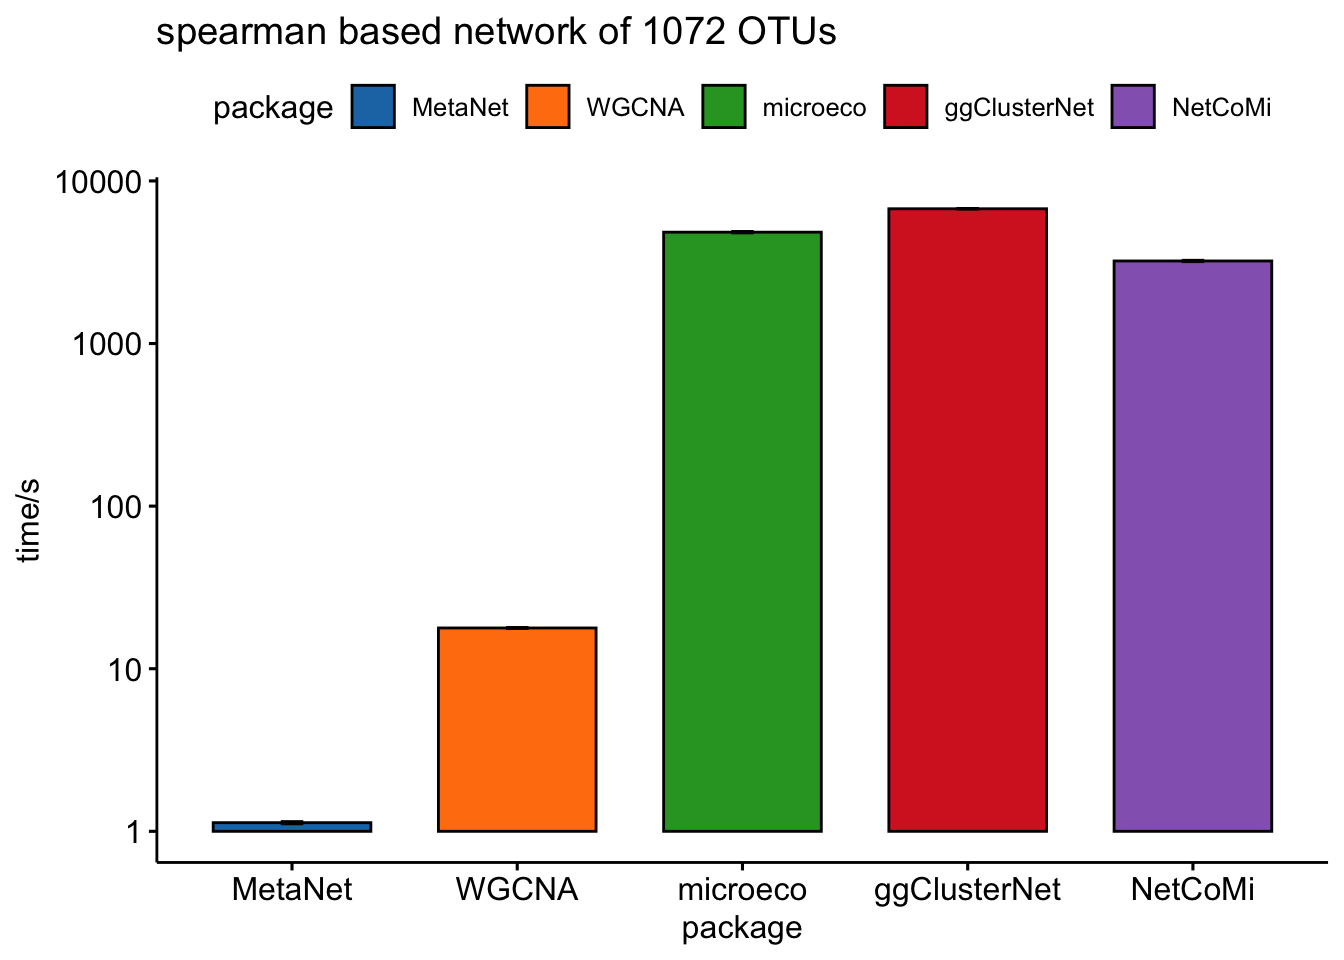
\includegraphics{_main_files/figure-latex/packages-comparison-1.pdf}
\caption{\label{fig:packages-comparison}network build of packages comparison}
\end{figure}

\hypertarget{distance}{%
\subsection{Distance}\label{distance}}

you can use \texttt{par\_sim()} to calculate various distance to get the pairwise similarity matrix.

\hypertarget{sparcc}{%
\subsection{SparCC}\label{sparcc}}

SparCC fits the Dirichlet distribution to the observed data, and iteratively calculates the proportion and correlation of species several times. The resulting correlation is the median of the distribution. \(p\)-values were calculated using the bootstrap method.This metric is said to be more useful with non-normal microbiome data.

\(D(x_i,x_j)=var(\log(\frac{x_i}{x_j}))\)

\texttt{par\_sparcc()} is available for SparCC calculation.

\hypertarget{others}{%
\subsection{Others}\label{others}}

There are some other methods available for network construction in \href{https://github.com/stefpeschel/NetCoMi}{\textbf{NetCoMi}}

\hypertarget{build-network}{%
\section{Build network}\label{build-network}}

\hypertarget{normally-build}{%
\subsection{Normally build}\label{normally-build}}

If you have done the \texttt{c\_net\_cal()}, you can get a network (igraph object) easily by \texttt{c\_net\_build()}. Some common attributes will be set automatically.

\begin{Shaded}
\begin{Highlighting}[]
\FunctionTok{c\_net\_build}\NormalTok{(corr,}\AttributeTok{r\_thres =} \FloatTok{0.6}\NormalTok{,}\AttributeTok{p\_thres =} \FloatTok{0.05}\NormalTok{,}\AttributeTok{del\_single =}\NormalTok{ T) }\OtherTok{{-}\textgreater{}}\NormalTok{ co\_net}
\NormalTok{co\_net}
\end{Highlighting}
\end{Shaded}

\begin{verbatim}
## IGRAPH 4639c34 UNW- 462 1401 -- 
## + attr: n_type (g/c), name (v/c), v_group (v/c), v_class (v/c), size
## | (v/n), label (v/c), shape (v/c), color (v/c), id (e/n), from (e/c),
## | to (e/c), weight (e/n), cor (e/n), p.adjust (e/n), p.value (e/n),
## | e_type (e/c), width (e/n), v_group_from (e/c), v_group_to (e/c),
## | e_class (e/c), color (e/c), lty (e/n)
## + edges from 4639c34 (vertex names):
## [1] s__un_f__Thermomonosporaceae--s__Actinocorallia_herbida    
## [2] s__un_f__Thermomonosporaceae--s__Kribbella_catacumbae      
## [3] s__un_f__Thermomonosporaceae--s__Kineosporia_rhamnosa      
## [4] s__un_f__Thermomonosporaceae--s__un_f__Micromonosporaceae  
## + ... omitted several edges
\end{verbatim}

\begin{Shaded}
\begin{Highlighting}[]
\FunctionTok{plot}\NormalTok{(co\_net)}
\end{Highlighting}
\end{Shaded}

\begin{figure}
\centering
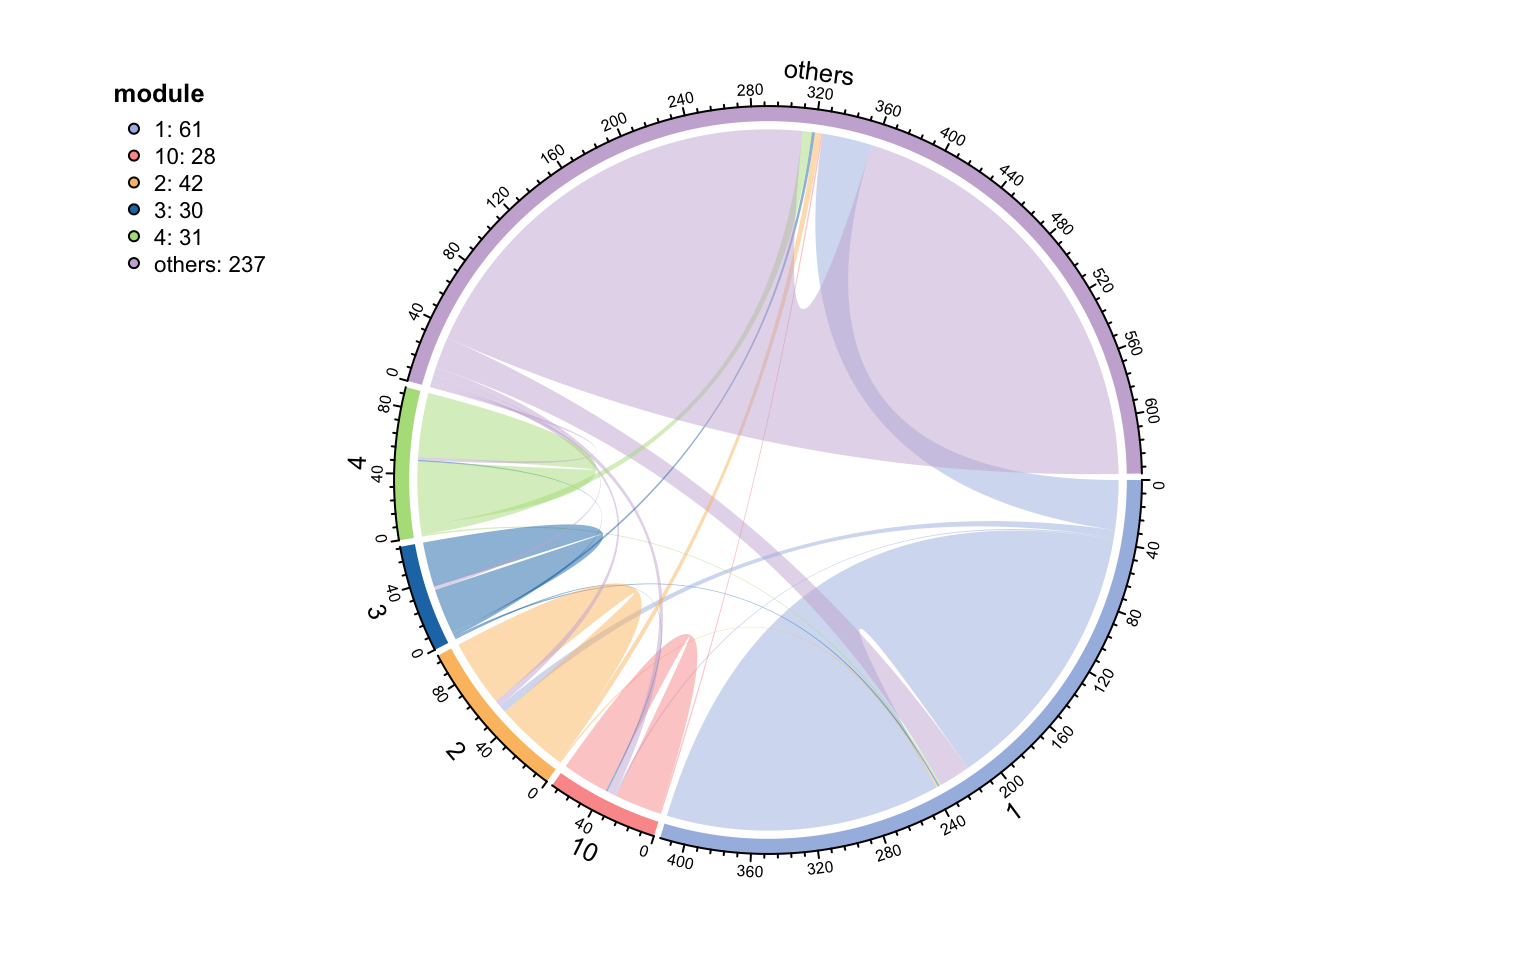
\includegraphics{_main_files/figure-latex/unnamed-chunk-8-1.pdf}
\caption{\label{fig:unnamed-chunk-8}Simple co-occurrence network}
\end{figure}

\begin{Shaded}
\begin{Highlighting}[]
\FunctionTok{c\_net\_build}\NormalTok{(corr2) }\OtherTok{{-}\textgreater{}}\NormalTok{ co\_net2}
\FunctionTok{plot}\NormalTok{(co\_net2)}
\end{Highlighting}
\end{Shaded}

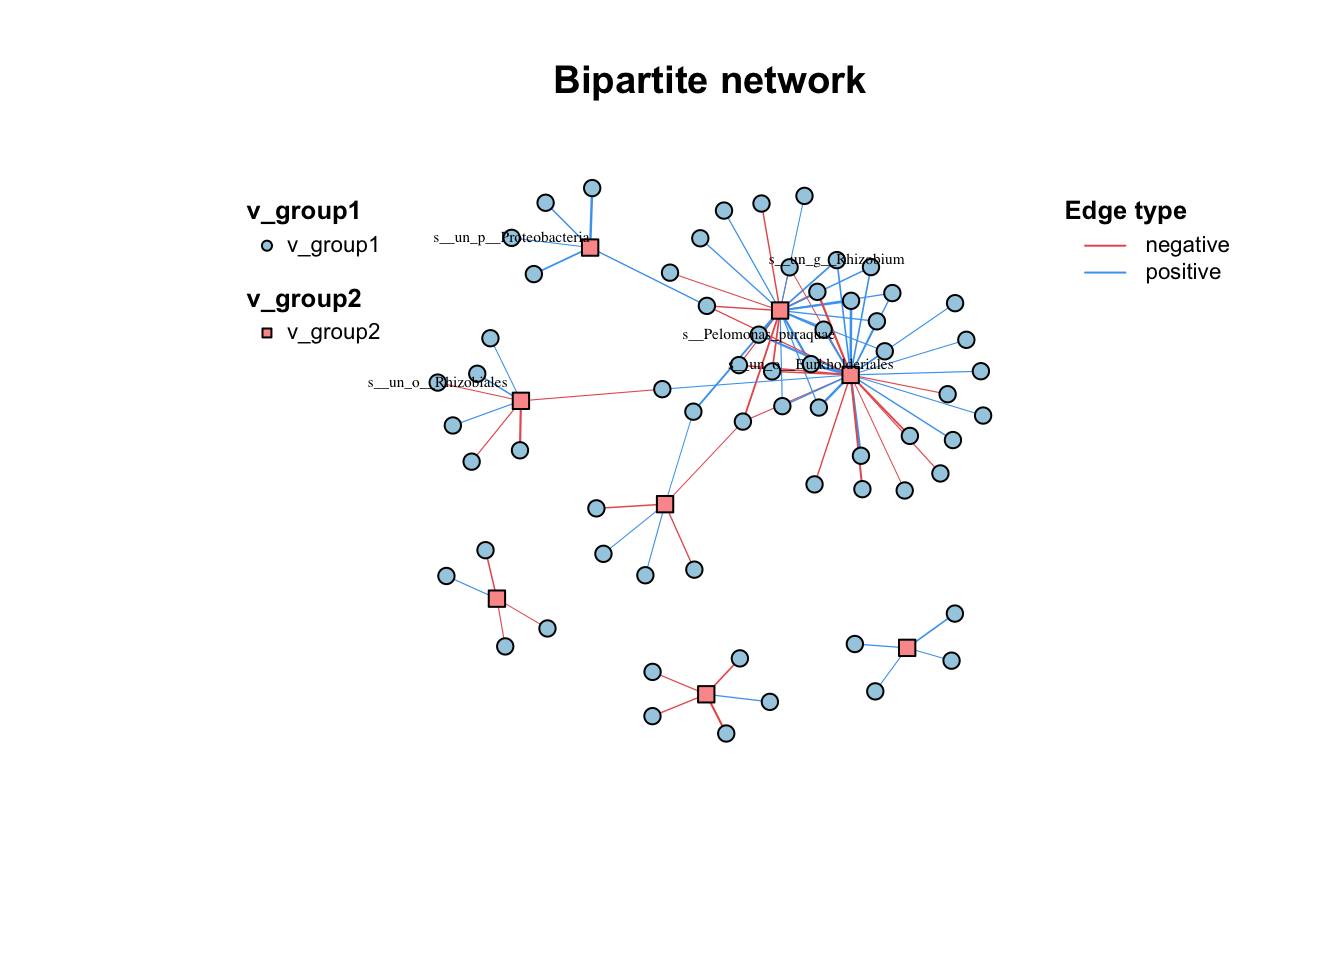
\includegraphics{_main_files/figure-latex/unnamed-chunk-9-1.pdf}
\#\#\# Multi-tables
When you have more than two tables for correlation network analysis, you can choose the \texttt{multi\_net\_build()} to calculate and build network. For subsequent multi-omics analysis, see Chapter \ref{multi-omics}.

\begin{Shaded}
\begin{Highlighting}[]
\FunctionTok{data}\NormalTok{(}\StringTok{"multi\_test"}\NormalTok{)}
\CommentTok{\#microbiome}
\FunctionTok{dim}\NormalTok{(micro)}
\DocumentationTok{\#\# [1] 18 50}
\CommentTok{\#metabolome}
\FunctionTok{dim}\NormalTok{(metab)}
\DocumentationTok{\#\# [1] 18 50}
\CommentTok{\#transcriptome}
\FunctionTok{dim}\NormalTok{(transc)}
\DocumentationTok{\#\# [1] 18 50}

\FunctionTok{multi\_net\_build}\NormalTok{(micro,metab,transc,}\AttributeTok{mode =} \StringTok{"full"}\NormalTok{,}\AttributeTok{method =} \StringTok{"spearman"}\NormalTok{,}\AttributeTok{filename =}\NormalTok{ F)}\OtherTok{{-}\textgreater{}}\NormalTok{multi1}

\FunctionTok{plot}\NormalTok{(multi1)}
\end{Highlighting}
\end{Shaded}

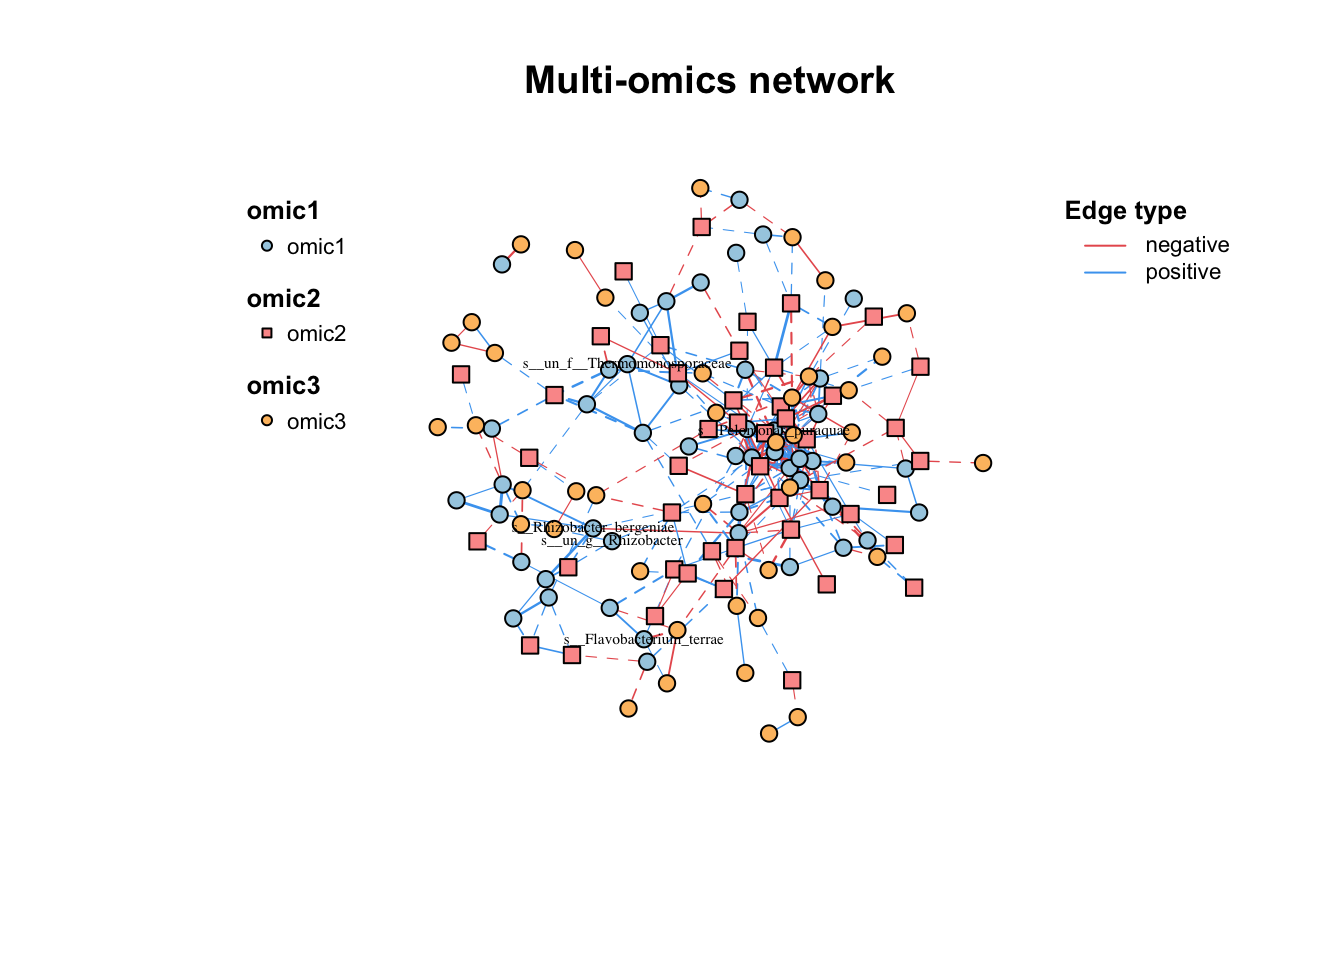
\includegraphics{_main_files/figure-latex/unnamed-chunk-10-1.pdf}
\#\#\# Edgelist
If you already get the pairwise relationship of data from other approaches (database), you can form it into a edgelist and use \texttt{c\_net\_from\_edgelist} to build network. It is useful for following analysis.

\begin{Shaded}
\begin{Highlighting}[]
\FunctionTok{load}\NormalTok{(}\StringTok{"../MetaNet/data/edgelist.rda"}\NormalTok{)}
\NormalTok{dnet}\OtherTok{=}\FunctionTok{c\_net\_from\_edgelist}\NormalTok{(arc\_count,}\AttributeTok{direct =}\NormalTok{ T)}
\FunctionTok{plot}\NormalTok{(dnet)}
\end{Highlighting}
\end{Shaded}

\begin{figure}
\centering
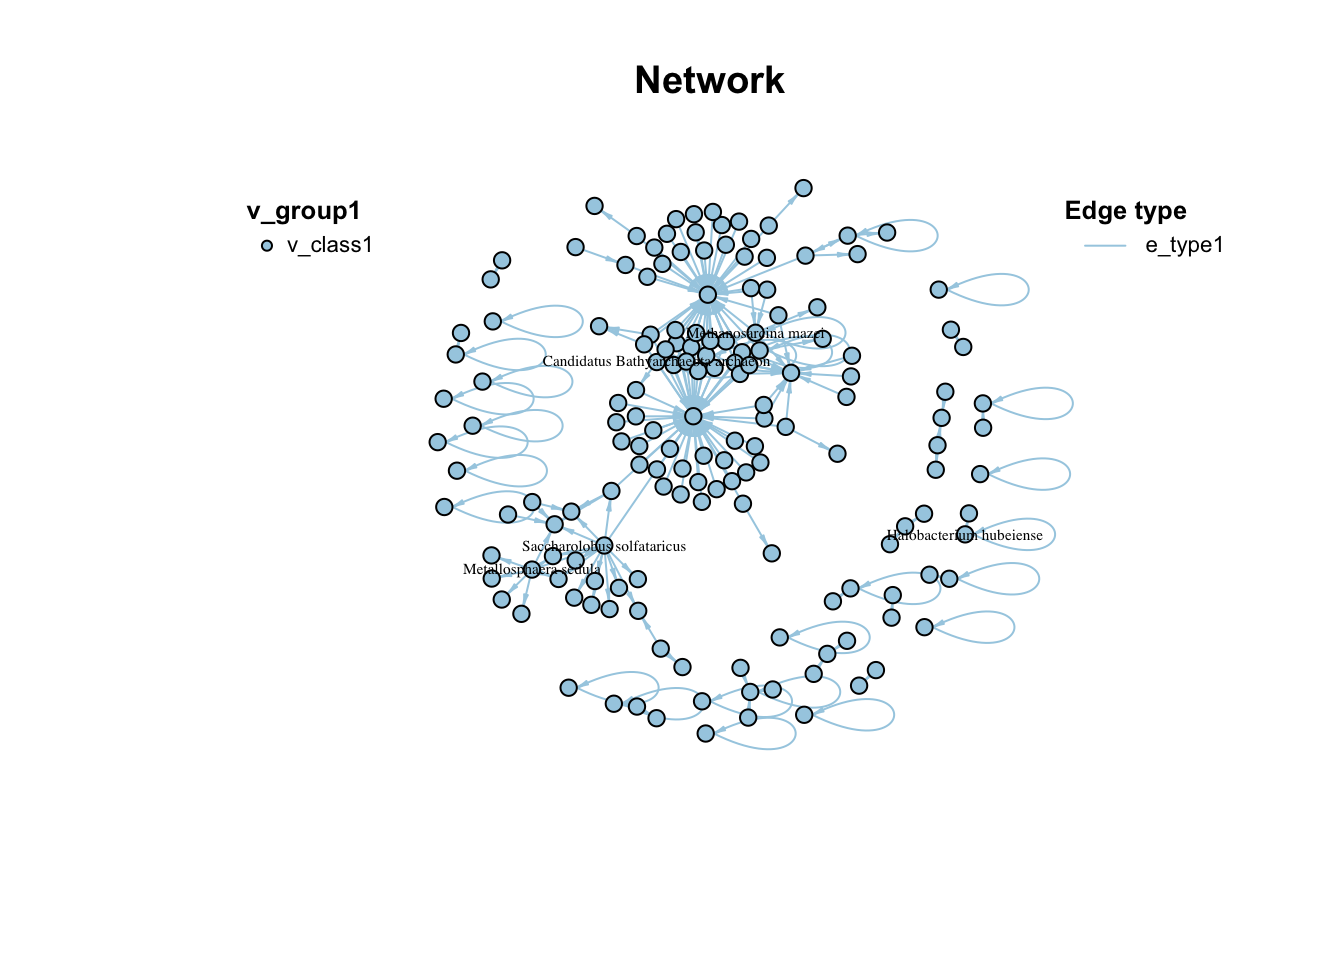
\includegraphics{_main_files/figure-latex/unnamed-chunk-11-1.pdf}
\caption{\label{fig:unnamed-chunk-11}Simple directed network}
\end{figure}

\hypertarget{rmt-optimize}{%
\section{RMT optimize}\label{rmt-optimize}}

The correlation-based relevance network method is most commonly used largely due to its simple calculation procedure and noise tolerance. However, most studies involving relevance network analysis use arbitrary thresholds (usually, we use r\textgreater0.6, p\textless0.05), and thus the constructed networks are subjective rather than objective.

This problem has been solved by a random matrix theory (RMT)-based approach (Figure \ref{fig:RMT}), which is able to automatically identify a threshold for cellular network construction from microarray data (\citet{dengMolecularEcologicalNetwork2012}).

\begin{figure}
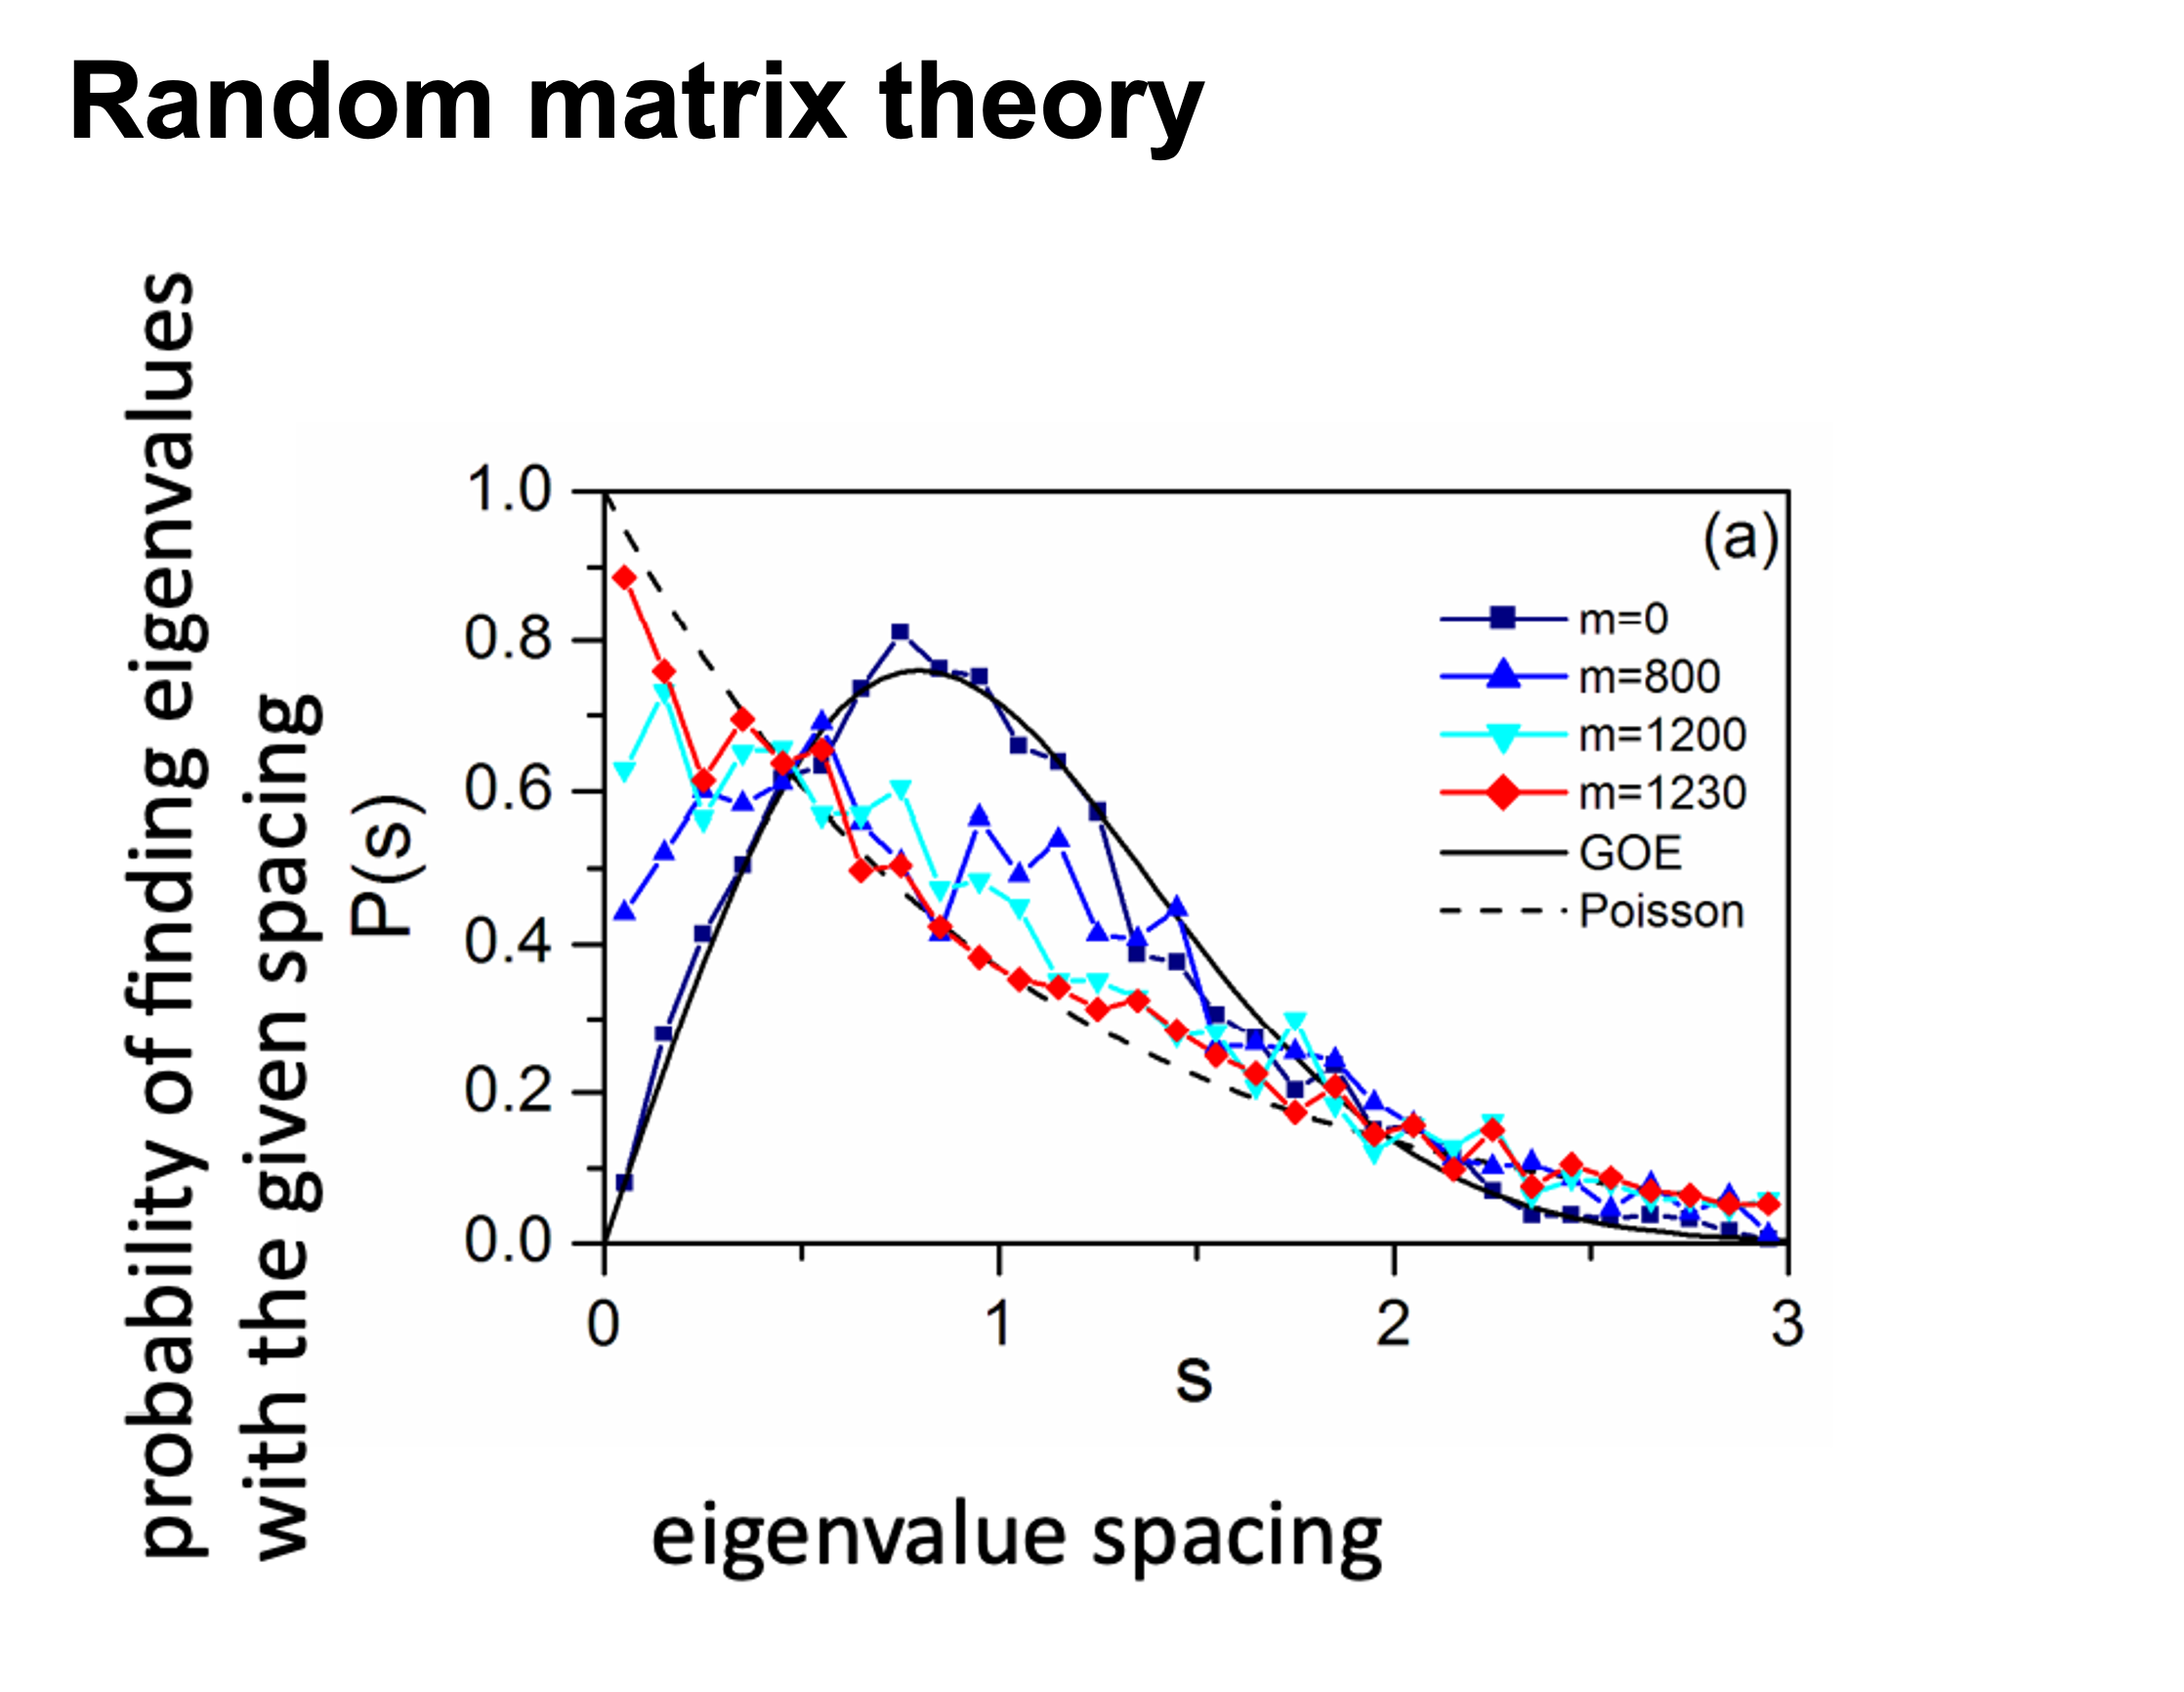
\includegraphics[width=5.59in]{images/2-1.RMT} \caption{random matrix theory (RMT)-based approach}\label{fig:RMT}
\end{figure}

use \texttt{RMT\_threshold()} , we can find the best r\_threshold to make the network with smallest noise.

the bigger log\_LE, less log\_LW, less log\_see, bigger p\_ks\_test indicate the better r\_threshold for a meaningful network construction.You can change the threshold range to calculate more finely.

\begin{Shaded}
\begin{Highlighting}[]
\FunctionTok{RMT\_threshold}\NormalTok{(corr}\SpecialCharTok{$}\NormalTok{r,}\AttributeTok{min\_threshold =} \FloatTok{0.5}\NormalTok{,}\AttributeTok{max\_threshold =} \FloatTok{0.9}\NormalTok{, }\AttributeTok{step =} \FloatTok{0.02}\NormalTok{)}\OtherTok{{-}\textgreater{}}\NormalTok{rmt\_res}
\DocumentationTok{\#\# =========================Calculating1:  threshold =0.5=========================}
\DocumentationTok{\#\# =========================Calculating2:  threshold =0.52=========================}
\DocumentationTok{\#\# =========================Calculating3:  threshold =0.54=========================}
\DocumentationTok{\#\# =========================Calculating4:  threshold =0.56=========================}
\DocumentationTok{\#\# =========================Calculating5:  threshold =0.58=========================}
\DocumentationTok{\#\# =========================Calculating6:  threshold =0.6=========================}
\DocumentationTok{\#\# =========================Calculating7:  threshold =0.62=========================}
\DocumentationTok{\#\# =========================Calculating8:  threshold =0.64=========================}
\DocumentationTok{\#\# =========================Calculating9:  threshold =0.66=========================}
\DocumentationTok{\#\# ========================Calculating10:  threshold =0.68========================}
\DocumentationTok{\#\# =========================Calculating11:  threshold =0.7=========================}
\DocumentationTok{\#\# ========================Calculating12:  threshold =0.72========================}
\DocumentationTok{\#\# ========================Calculating13:  threshold =0.74========================}
\DocumentationTok{\#\# ========================Calculating14:  threshold =0.76========================}
\DocumentationTok{\#\# ========================Calculating15:  threshold =0.78========================}
\DocumentationTok{\#\# =========================Calculating16:  threshold =0.8=========================}
\DocumentationTok{\#\# ========================Calculating17:  threshold =0.82========================}
\DocumentationTok{\#\# ========================Calculating18:  threshold =0.84========================}
\DocumentationTok{\#\# ========================Calculating19:  threshold =0.86========================}
\DocumentationTok{\#\# The Intermediate files saved in ./RMT\_temp/ .}
\FunctionTok{plot}\NormalTok{(rmt\_res)}
\end{Highlighting}
\end{Shaded}

\begin{figure}
\centering
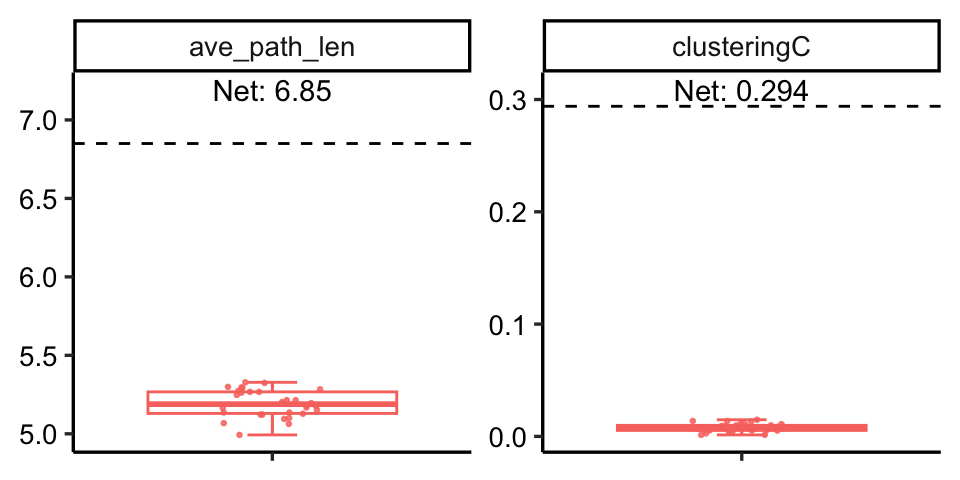
\includegraphics{_main_files/figure-latex/unnamed-chunk-12-1.pdf}
\caption{\label{fig:unnamed-chunk-12}RMT\_threshold result from 0.5 to 0.9}
\end{figure}

\begin{verbatim}
## [1] "recommend r_threshold:  0.835"
## [1] 0.835
\end{verbatim}

You can set the \texttt{gif=T} in \texttt{RMT\_threshold} and get a gif file to observe the distribution of eigenvalue spacing for different r-thresholds.

\texttt{r\ if\ (knitr::is\_html\_output())\ \textquotesingle{}\ !{[}(\textbackslash{}\#fig:unnamed-chunk-13)the\ distribution\ of\ eigenvalue\ spacing\ from\ 0.5\ to\ 0.9{]}(images/rmt\_nnsd.gif)\ \ \textquotesingle{}}

\hypertarget{manipulation}{%
\chapter{Manipulation}\label{manipulation}}

\hypertarget{attributes}{%
\section{Attributes}\label{attributes}}

get\_v
get\_e
get\_n

\hypertarget{annotation}{%
\section{Annotation}\label{annotation}}

anno\_vertex
anno\_edge

summ2col

\hypertarget{filter-sub-net}{%
\section{Filter (Sub-net)}\label{filter-sub-net}}

c\_net\_filter

\hypertarget{export}{%
\section{Export}\label{export}}

c\_net\_save

\hypertarget{visualization}{%
\chapter{Visualization}\label{visualization}}

\hypertarget{basic-plot}{%
\section{Basic plot}\label{basic-plot}}

\hypertarget{layout}{%
\section{Layout}\label{layout}}

\hypertarget{other-styles}{%
\section{Other styles}\label{other-styles}}

\hypertarget{ggplot}{%
\subsection{ggplot}\label{ggplot}}

\hypertarget{gephi}{%
\subsection{Gephi}\label{gephi}}

\hypertarget{cytoscape}{%
\subsection{Cytoscape}\label{cytoscape}}

\hypertarget{topology}{%
\chapter{Topology}\label{topology}}

\hypertarget{complex-network}{%
\section{Complex network}\label{complex-network}}

The microbial co-occurrence network we study is a complex network, which generally has the following characteristics, scale-free, small-world attributes, modularity and hierarchy.

\begin{longtable}[]{@{}
  >{\raggedright\arraybackslash}p{(\columnwidth - 2\tabcolsep) * \real{0.0314}}
  >{\raggedright\arraybackslash}p{(\columnwidth - 2\tabcolsep) * \real{0.9686}}@{}}
\caption{Common characteristic}\tabularnewline
\toprule()
\endhead
\textbf{Terminology} & \textbf{Explanation} \\
\textbf{Scale-free} & Scale-free It is a most notable characteristic in complex systems. It was used to desibe the finding that most nodes in a network have few neighbors while few nodes have large amount of neighbors. In most cases, the connectivity distribution asymptotically follows a power law. It can be expressed in , where \(P(k) \sim k^{-y}\) P(k) is the number of nodes with k degrees, k is connectivity/degrees andγis a constant. \\
\textbf{Small-world} & Small-world It is a terminology in network analyses to depict the average distance between nodes in a network is short, usually logarithmically with the total number of nodes. It means the network nodes are always closely related with each other. \\
\textbf{Modularity} & The modularity of a graph with respect to some division (or vertex types) measures how good the division is, or how separated are the different vertex types from each other. It defined as

\(Q=\frac{1}{2m} \sum_{i,j} (A_{ij}-\gamma\frac{k_i k_j}{2m})\delta(c_i,c_j)\)

here m\emph{m} is the number of edges, \(A_{ij}\) is the element of the \emph{A} adjacency matrix in row \emph{i} and column \emph{j}, \(k_i\) is the degree of i, \(k_j\) is the degree of \emph{j}, \(c_i\) is the type (or component) of \emph{i}, \(c_j\) that of \emph{j}, the sum goes over all \emph{i} and \emph{j} pairs of vertices, and \(\delta(x,y)\) is 1 if \emph{x}=\emph{y} and 0 otherwise. The resolution parameter \(\gamma\) allows weighting the random null model, which might be useful when finding partitions with a high modularity.The original definition of modularity is retrieved when setting \(\gamma\) to 1. \\
\textbf{Hierarchy} & Hierarchy It was used to depict the networks which could be arranged into a hierarchy of groups representing in a tree structure. Several studies demonstrated that metabolic networks are usually accompanied by a hierarchical modularity. \\
\bottomrule()
\end{longtable}

\texttt{fit\_power()} is used to prove the scale-free. \texttt{smallworldness()} can calculate the smallworld index.

\hypertarget{topology-indexes}{%
\section{Topology indexes}\label{topology-indexes}}

\begin{longtable}[]{@{}
  >{\raggedright\arraybackslash}p{(\columnwidth - 6\tabcolsep) * \real{0.0893}}
  >{\raggedright\arraybackslash}p{(\columnwidth - 6\tabcolsep) * \real{0.1039}}
  >{\raggedright\arraybackslash}p{(\columnwidth - 6\tabcolsep) * \real{0.3474}}
  >{\raggedright\arraybackslash}p{(\columnwidth - 6\tabcolsep) * \real{0.4594}}@{}}
\toprule()
\begin{minipage}[b]{\linewidth}\raggedright
Indexes
\end{minipage} & \begin{minipage}[b]{\linewidth}\raggedright
Formula
\end{minipage} & \begin{minipage}[b]{\linewidth}\raggedright
Note
\end{minipage} & \begin{minipage}[b]{\linewidth}\raggedright
Description
\end{minipage} \\
\midrule()
\endhead
\textbf{Part I: network indexes for individual nodes} & & & \\
Connectivity/ Degree (centrality) & \(k_i=\sum_{j\neq i}a_{ij}\) & 𝑎𝑖𝑗 is the connection strength between nodes i and j. when 𝑎𝑖𝑗=1, ki is the unweighted degree & It is also called node degree. It is the most commonly used concept for describing the topological property of a node in a network. \\
Betweenness centrality & \(B_i=\sum_{j,k}\frac{\sigma(i,j,k)}{\sigma(j,k)}\) & 𝜎(𝑗,𝑖,𝑘) is the number of shortest paths between nodes j and k that pass through node i. 𝜎(𝑗,𝑘) is the total number of shortest paths between j and k. & It is used to describe the ratio of paths that pass through the ith node. High Betweenness node can serve as a broker similar to stress centrality. \\
Closeness centrality & \(Ci=1/\sum_{i\neq j}d_{ij}\) & The closeness centrality of a vertex is defined as the inverse of the sum of distances to all the other vertices in the graph. dij is the shortest distances from node i to j. & Closeness centrality measures how many steps is required to access every other vertex from a given vertex. \\
Eigenvector centrality & \(EC_i=\frac{1}{\lambda}\sum_{j\in M(i)}EC_j\) & M(𝑖) is the set of nodes that are connected to the ith node and λ is a constant eigenvalue. & It is used to describe the degree of a central node that it is connected to other central nodes. \\
Clustering coefficient & \(CCo_i=\frac{2l_i}{k_i'(k_i'-1)}\) & li is the number of links between neighbors of node i and k i ' is the number of neighbors of node i. & It describe how well a node is connected with its neighbors. If it is fully connected to its neighbors, the clustering coefficient is 1. A value close to 0 means that there are hardly any connections with its neighbors. It was used to describe hierarchical properties of networks. \\
Eccentricity & \(E_i=\max_{j\neq i}(d_{ij})\) & dij is the shortest distance from node i to node j & The eccentricity of a vertex is its shortest path distance from the farthest other node in the graph. \\
Page.rank & \(PR_i=\sum_{j\in B_i}\frac{PR_j}{l_j}\) & i is the node whose pr value needs to be calculated, and Bi is the set of all nodes pointing to node i. PRj is the pr value of node j and lj is the number of links between neighbors of node j. & Calculates the Google PageRank for the specified vertices. PageRank, or webpage ranking, also known as webpage level, is an indicator to measure the importance of webpages. \\
Kleinberg's hub and authority centrality & \(HC=\lambda_{AA^T}\) \(AC=\lambda_{A^TA}\) & The hub scores of the vertices are defined as the principal eigenvector of AAT, the authority scores of the vertices are defined as the principal eigenvector of ATA. where A is the adjacency matrix of the graph. & A node is an authority if it is linked to by hubs; it is a hub if it links to authorities. \\
\textbf{Part II: The overall network topological indexes} & & & \\
Average connectivity/ degree & \(\overline{k}=\frac{\sum_{i=1}^{n}k_i}{n}\) & k i is degree of node i and n is the number of nodes. & Higher avgK means a more complex network. \\
Average path length/ Average geodesic distance & \(L=\frac{\sum_{i \ne j}d_{ij}}{n(n-1)}\) & dij is the shortest path between node i and j. & A smaller GD means all the nodes in the network are closer. \\
global efficiency/ Geodesic efficiency & \(E_g=\frac{\sum_{i \ne j}1/d_{ij}}{n(n-1)}\) & all parameters shown above. & It is the opposite of GD. A higher E means that the nodes are closer. \\
Centralization of degree & \(CD=\sum_{i=1}^{n}(\max(k)-k_i)\) & max(k) is the maximal value of all connectivity values and k i represents the connectivity of ith node. Finally this value is normalized by the theoretical maximum centralization score. & It is close to 1 for a network with star topology and in contrast close to 0 for a network where each node has the same connectivity. \\
Centralization of betweenness & \(CB=\sum_{i=1}^{n}(\max(B)-B_i)\) & max(B) is the maximal value of all betweenness values and B i represents the betweenness of ith node. Finally this value is normalized by the theoretical maximum centralization score. & It is close to 0 for a network where each node has the same betweenness, and the bigger the more difference among all betweenness values. \\
Centralization of closeness & \(CC=\sum_{i=1}^{n}(\max(C)-C_i)\) & max(C) is the maximal value of all closeness values and Ci represents the closeness of ith node. Finally this value is normalized by the theoretical maximum centralization score. & It is close to 0 for a network where each node has the same closeness, and the bigger the more difference among all closeness values. \\
Centralization of eigenvector centrality & \(CE=\sum_{i=1}^{n}(\max(EC)-EC_i)\) & max(EC) is the maximal value of all eigenvector centrality values and EC i represents the eigenvector centrality of ith node. Finally this value is normalized by the theoretical maximum centralization score. & It is close to 0 for a network where each node has the same eigenvector centrality, and the bigger the more difference among all eigenvector centrality values. \\
Density & \(D=\frac{2l}{n(n-1)}\) & l is the sum of total links. & The density of a graph is the ratio of the number of edges and the number of possible edges. It is closely related to the average connectivity. \\
Average clustering coefficient & \(\overline{CCo}=\frac{\sum_{i=1}^{n}CCo_i}{n}\) & 𝐶𝐶oi is the clustering coefficient of node i. & It is used to measure the extent of module structure present in a network. \\
Transitivity & \(Tr=\frac{\sum_{i=1}^{n}2l_i}{\sum_{i=1}^{n}(k'_i)(k'_i-1)}\) & li is the number of links between neighbors of node i and k i ' is the number of neighbors of node i. & Sometimes it is also called the entire clustering coefficient. It has been shown to be a key structural property in social networks. \\
Natural connectivity & \(NC=\ln{\left(\frac{1}{N}\sum_{i=1}^{N}e^{\lambda_i}\right)}\) & Where N is nodes number of the network, represents the eigenvalue of the network adjacency matrix. & \\
\bottomrule()
\end{longtable}

\hypertarget{stability}{%
\chapter{Stability}\label{stability}}

It is very important to compare networks stability based on different groups. So MetaNet collects lots of methods to reflect the stability and complexity, these algorithms are coded using Parallel Computing which can be much faster.

\hypertarget{robustness-tests}{%
\section{Robustness tests}\label{robustness-tests}}

Robustness tests of networks were done with natural connectivity as it can reflect the stability of networks (\citet{wujunNaturalConnectivityComplex2010}). Specifically, natural connectivity was calculated after removing the nodes (remove five nodes from a network at one time until 70\% of nodes disappear), and the downtrend level of natural connectivity indicated the connectivity performance of the network after being damaged to a certain extent.

\hypertarget{community-stability}{%
\section{Community stability}\label{community-stability}}

Community stability can be characterized by various indexes, such as \textbf{robustness}, \textbf{vulnerability} and \textbf{cohesion}. Networks with higher robustness and lower vulnerability tend to be more stable (\citet{yuanClimateWarmingEnhances2021}).
Also, community stability is commonly associated with negative interactions, and high percentage of negative correlations within communities is essential for maintaining a stable ecological system.
\#\#\# Robustness
The robustness was regarded as when 50\% of nodes were randomly removed and results were based on 100 repetitions of the simulation.

\hypertarget{vulnerability}{%
\subsection{Vulnerability}\label{vulnerability}}

To evaluate the speed of disturbance spreading within a network, the global efficiency was regarded as the average of the efficiency over all pairs of nodes, which was calculated by the number of edges in the shortest path between paired nodes. The vulnerability, which reflected the relative contribution of each node to the globe efficiency, was represented by the maximal vulnerability of nodes in the network.

\hypertarget{cohesion}{%
\subsection{Cohesion}\label{cohesion}}

Cohesion was calculated to quantify the connectivity of microbial communities in each group. Cohesion contains both positive and negative cohesion values, which indicate that associations between taxa attributed to positive and negative species interactions as well as similarities and differences in niches of microbial taxa11. Briefly, pairwise Pearson correlation matrix across taxa was calculated based on abundance-weighted matrix. After ``taxa shuffle'' null module-correcting with 200 simulations, average positive and negative correlations was calculated to get a connectedness matrix. Finally, positive and negative cohesions were calculated for each sample respectively by multiplying the abundance-weighted matrix and connectedness matrix. The absolute value of negative: positive cohesion is an important index for community stability.
\(cohesion=\sum_{i=1}^{m}{{\rm abundance}_i\times connectness}_i\)

\hypertarget{multi-omics}{%
\chapter{multi-omics}\label{multi-omics}}

\hypertarget{case-study}{%
\section{Case study}\label{case-study}}

In-depth multi-omic profiling was performed on each sample including plasma proteomics (targeted and untargeted), metabolomics (untargeted), lipidomics (semi-targeted), and gene expression (transcriptomics) from peripheral blood mononuclear cells (PBMCs).(\citet{contrepoisMolecularChoreographyAcute2020})

\begin{figure}
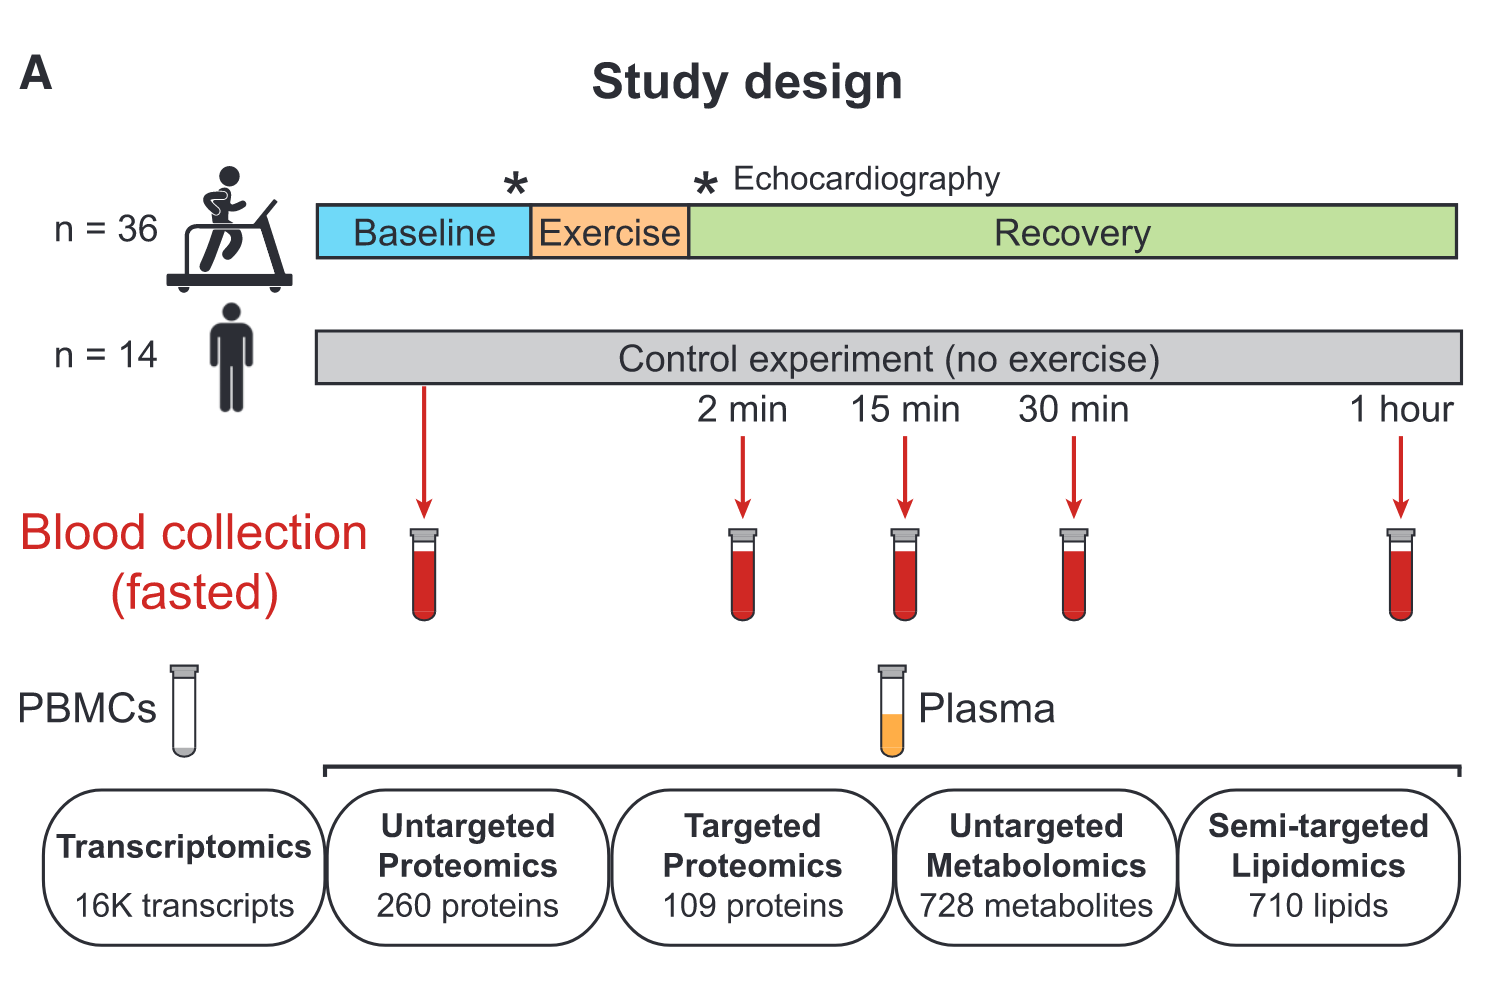
\includegraphics[width=2.51in]{images/7-1.cell_study} \caption{Overview of the study design including an acute bout of exercise}\label{fig:cell-study}
\end{figure}

  \bibliography{book.bib,packages.bib,network.bib}

\end{document}
